\documentclass{report}
\usepackage[T1]{fontenc}
\usepackage{graphicx}
\usepackage[top=1in, bottom=1in, right=1in, left=1in]{geometry}

\begin{document}
	\fontfamily{lmtt}\selectfont
	\begin{flushleft}
	\section*{Introduction}
	\vspace{-0.1cm}\hrule\vspace{0.2cm}
	\par{Flowcell sensors have many applications; disease detection, refractive index measuring, and reactivity measurements to name a few. These sensors have been operating on the basis of electromagnetic surface phenomena for decades. Most flowcells on the market work by exploiting surface plasma oscillations (SPOs). These oscillations are highly sensitive to changes in the optical properties of the adjacent medium and follow from Maxwell's equations when the dielectric functions of each medium satisfies 
	\[
		\frac{\epsilon_{spo}}{\epsilon_{adjacent}} < -1
	\]
	Metals like aluminum, copper, gold, and silver have negative dielectric functions at wavelengths in the red/infrared, so films of these metals are used as the source of SPOs in most flowcell sensors. There are quite a few drawbacks for using metal films, however. Metals are highly reactive so regular maintenance is necessary. These films also require particular wavelengths of incident light to excite the oscillations. Rather than using metal films, one-dimensional photonic crystals, or multilayers, can be designed to exhibit the phenomenon of surface electromagnetic waves (SEW) or Bloch surface waves (BSW), named after the physicist Felix Bloch who was famous for working with periodic systems. These surface waves have the same practical application as SPOs. Multilayers overcome both of the shortcomings of metal films listed here. They can be designed to work for any wavelength and are typically made of nonreactive glass. In addition to these benefits, we expect that our 3-D printed and robust, multilayer-based, flowcell sensor will be more sensitive and precise with its measurements and be far cheaper to both build and maintain.}
	\section*{Theory}
	\vspace{-0.1cm}\hrule\vspace{0.2cm}
	\par{In a metal incident light of a certain frequency $\omega_p$, the plasma frequency, can excite surface electrons and cause them to begin oscillating. These electrons are bound to the surface and hence the oscillations occur on the surface. By putting a thin piece of metal foil on the hypotenusal side of a prism these surface modes can be excited by shining light through the prism and onto the interface. When the light is just totally internally reflected, a strong evanescent field forms on the interface and a surface wave propagates parallel to the interface. This field can excite the electrons if the parallel component of the wave vector (i.e. the momentum of the photons travelling along the interface) satisfies the dispersion relation}
\[
	K(\omega_p) = \frac{\omega_p}{c} \sqrt{\frac{\epsilon_1\epsilon_2\mu_1\mu_2}{\epsilon_1\mu_1 + \epsilon_2\mu_2}}
\]
	\par{then the electrons will absorb the photons that would have undergone TIR and begin resonating. If one looks at the reflected image from the beam a dark band, representing the decreased intensity in the reflected power due to absorption, appears.}
	\par{A practically equivalent situation an be created by utilizing a 1D photonic crystal, or \textit{multilayer}. When analyzing the reflected power of an SPR system, a very sharp dip in reflectivity occurs at the resonant angle due to absorption. Multilayers can be designed to exhibit the very same dip in reflectivity. When using a multilayer instead of a metal film, the sharp dip in reflectivity is actually the coupling of the incident light to a surface wave mode. For a given wavelength of light, there is a certain angle of incidence corresponding to this mode. That angle is a function of the index of refraction in the transmitting medium. So, if the index of the transmitting medium varies, the dark band in the reflected image will also vary. It is important to note that their are several benefits to using the multilayer setup rather than an SPR setup. Firstly the multilayer can be designed so that incident light of \textit{any} wavelength couples to the SEW mode. Second the strength of the SEW fields are much higher with the multilayer setup, resulting in greater sensitivity. Finally, the multilayer can be built out of non-reactive glasses providing a much more robust chip which is easy to maintain.\\
	References:\\
	``Electromagnetic propagation in periodic stratified media. I. General Theory" Yeh, Yariv, Hong (1977)\\
	``Optical surface waves in periodic layered media" Yeh, Yariv (1978)\\
	``Experimental Measurement of the Effect of Termination on Surface Electromagnetic Waves in One-Dimensional Photonic Bandgap Arrays" Robertson (1999)\\
	``Surface plasmon-like sensor based on surface electromagnetic waves in a photonic band-gap material" Shinn, Robertson (2004)\\
	``Biosensing using surface electromagnetic waves in photonic band gap multilayers" Farmer, Robertson (2012)\\
	}
	\section*{Experimental Design}
	\vspace{-0.1cm}\hrule\vspace{0.2cm}
	\par{Our sensor is composed of a three primary parts: a central stage on which the prism and flowcell chamber are mounted and coupled together, and two rotating arms; one holds a laser (and a lens to focus it), the other holds the CCD for picking up the reflected image. The central stage is a round, two-tiered device with four holes on the top tier so that the flowcell baseplate can be attached. A channel for attaching the beam arms wraps around the top tier, with a sheared opening in the back so that the beam connectors can be attached easily. This channel keeps the beams firmly in place but also allows them to rotate around the main stage when enough force is applied due to the snug fit of the beam connectors. The housing of the laser, lens, and CCD were all 3D printed.\\}
	\vspace{0.5cm}
	\begin{figure}[h]
		\centering
		\raisebox{-0.5\height}{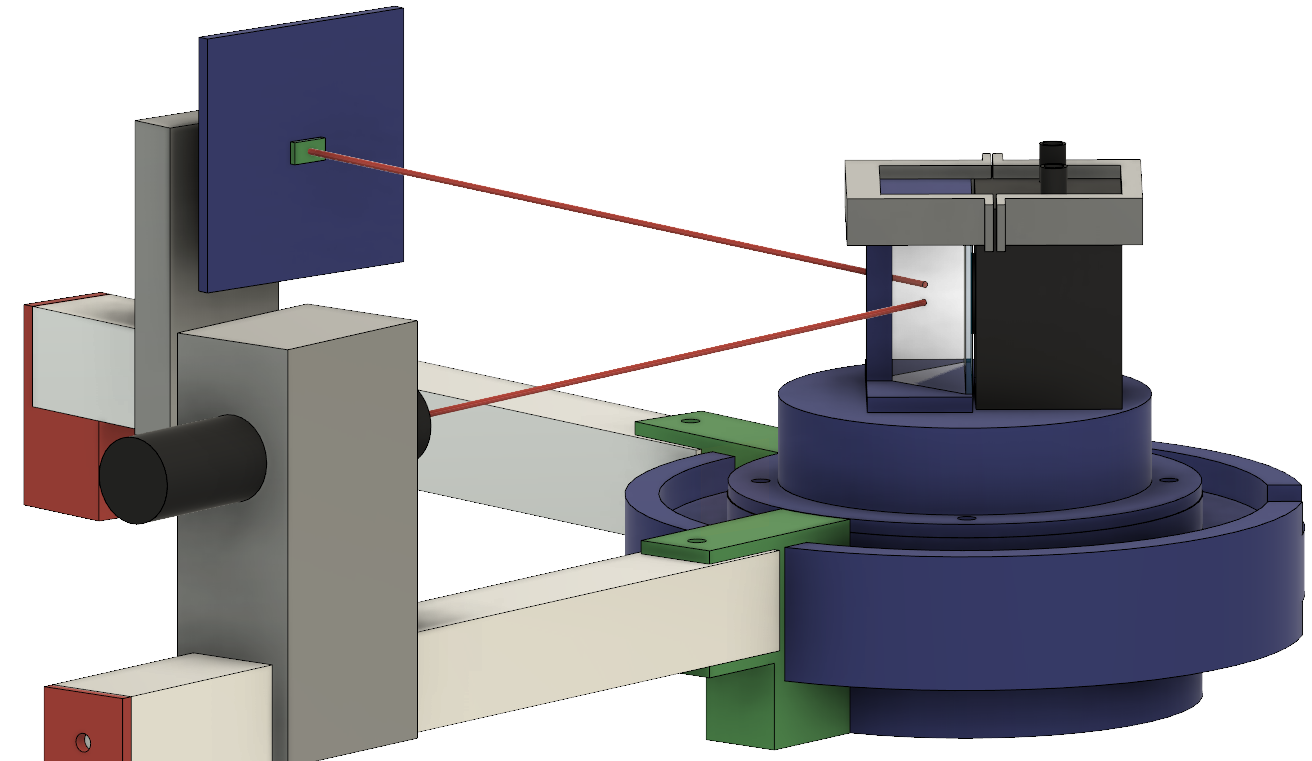
\includegraphics[scale=0.35]{media/setup_ccdview.PNG}}
		\raisebox{-0.5\height}{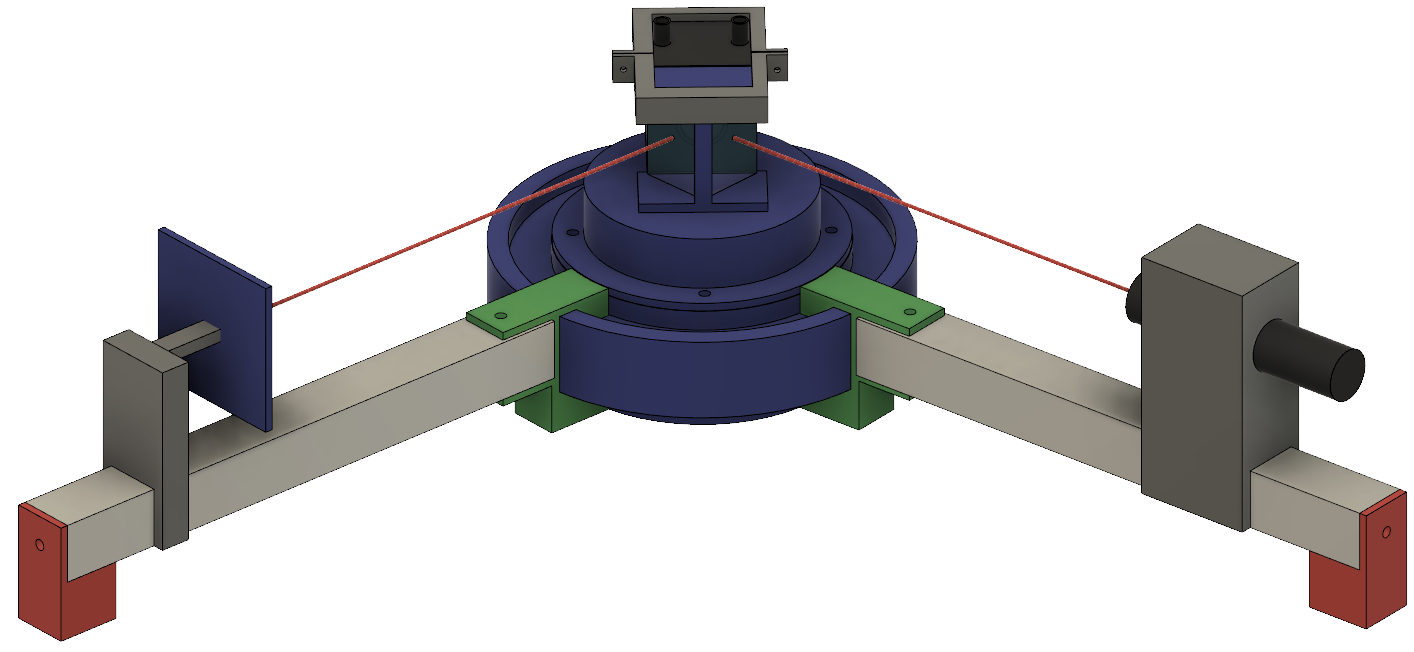
\includegraphics[scale=0.35]{media/setup_frontalview.PNG}}
		\raisebox{-0.5\height}{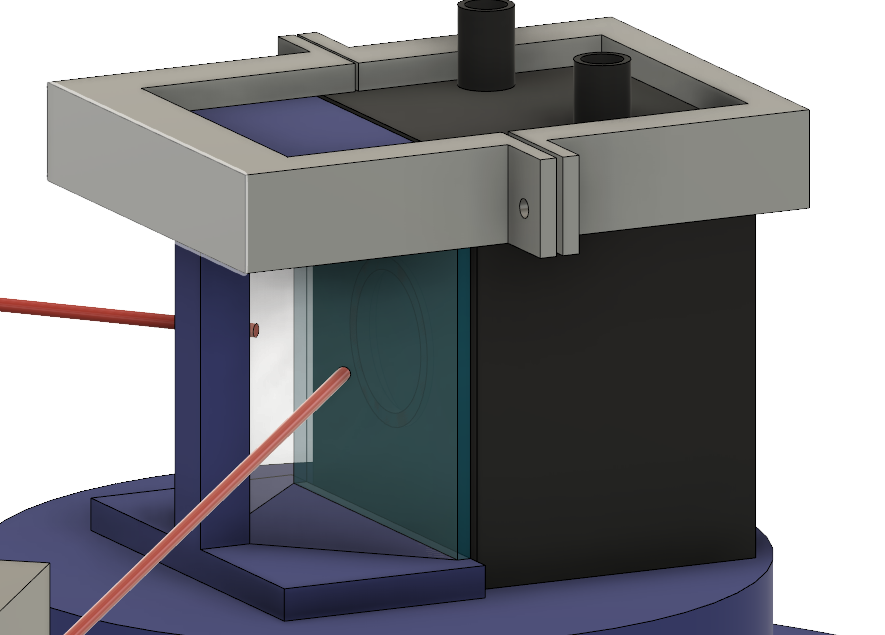
\includegraphics[scale=0.35]{media/setup_prism-multilayerview.PNG}}
	\end{figure}
	
	\section*{Software Design}
	\vspace{-0.1cm}\hrule\vspace{0.2cm}
	A vital part in using our flowcell is capturing data during a run and analyzing that data. To do this I have created a program that captures video from the CCD and processes that data in real time to display the index of refraction within the flowcell chamber.\\
	The program was built with the Electron package from the Node.js framework. This package uses the popular web-languages HTML, Javascript, and CSS. Electron provides programs access to more hardware than web browsers resulting in clean, styled, and fast programs.
	\section*{Methods}
	\vspace{-0.1cm}\hrule\vspace{0.2cm}
	\section*{Results}
	\vspace{-0.1cm}\hrule\vspace{0.2cm}
	TBD\\
	\section*{Conclusions}
	\vspace{-0.1cm}\hrule\vspace{0.2cm}
	TBD\\
	\pagebreak
	Some figures to use in the paper
	\end{flushleft}
\end{document}